%
% WebUI
%

\chapter{WebUI}
\label{webui}

{\em pDLNA} includes a small WebUI, which is accessable via the following URL \verb|http://ListenIPAddress:HTTPPort/webui/|.

\begin{colframeimportantnote}
\textsc{IMPORTANT NOTE:} If your client's IP address, which you would like to use to access the WebUI, is not included in the {\em AllowedClients} configuration parameter, you will not be able to access it.
\end{colframeimportantnote}

This small WebUI gives the chance to navigate through the indexed media items, have a detailed look on connected {\em UPnP} and {\em DLNA} devices and determine some process information like memory usage, the amount and size of indexed media items in the database or even the supported codecs of your \verb|FFmpeg| installation.

The WebUI does have a navigation part (coloured in blue) on the left side of the website. The information itself will be shown on the right side (coloured in white). The navigation is split in three different sections, which will be described in the following three sections.

\section{Configured media}

The screenshot in figure~\ref{fig:webgui-landingpage} shows the landing page of the WebUI, which show the root directory of the media library. It also shows the external media items (if any), which might be configured in the configuration file (see section~\ref{configExternal}). In the navigation of the WebUI, in the {\em Configured media} section, all in the configuration file configured directories (see section~\ref{configDirectory}) are listed. The number in the brackets after the directory name gives the information, how much items are in this specific directory.

\begin{figure}[!ht]
	\centering
		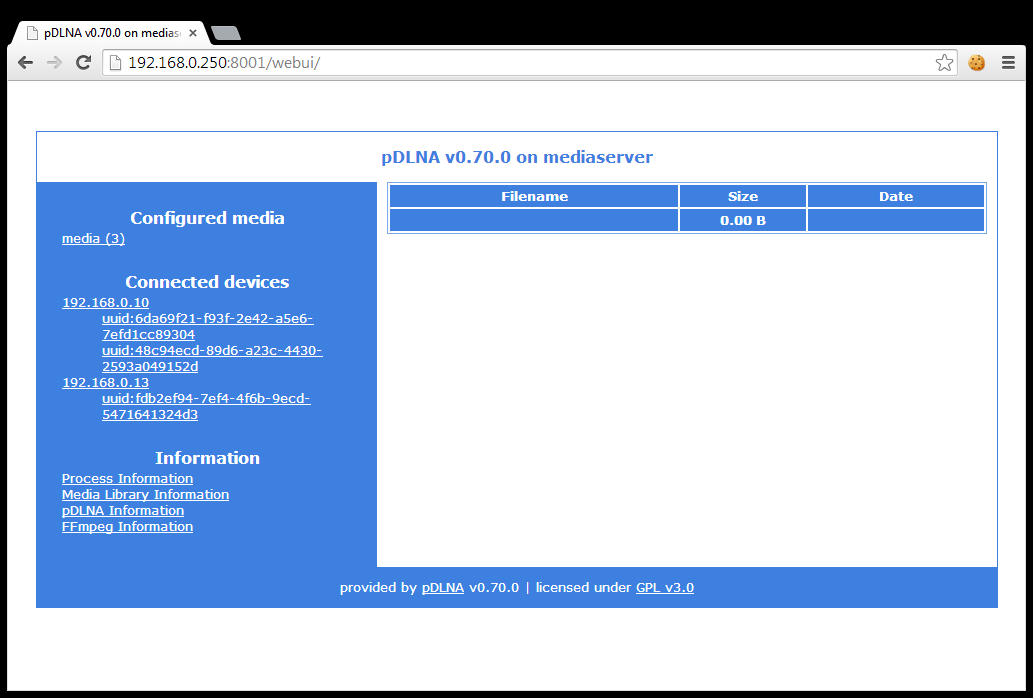
\includegraphics[width=34em]{images/webui_content_landing}
	\label{fig:webgui-landingpage}
	\caption{WebUI: Landing page}
\end{figure}

By clicking (in this case) on the {\em media} directory, the directory tree will be shown as it appears in figure~\ref{fig:webgui-audio}. With an additional click on the {\em audio} directory, the files, which are in this directory will be shown in the content part of the WebUI. The content table, as can be seen, shows the information about the filename, the size and the date of the media file.

\begin{figure}[!ht]
	\centering
		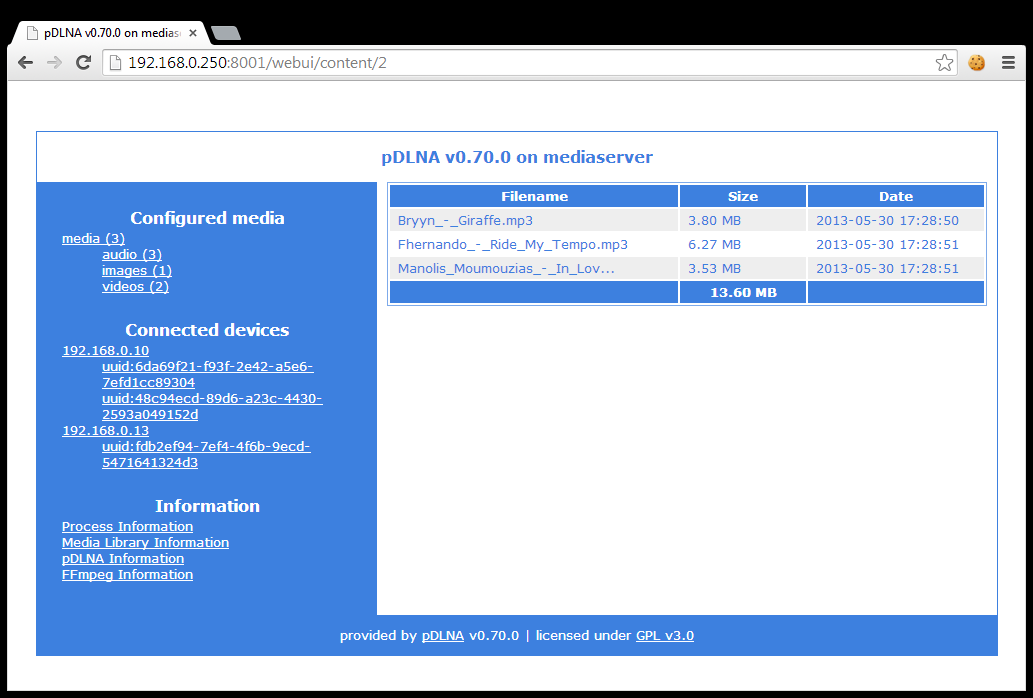
\includegraphics[width=34em]{images/webui_content_audio}
	\label{fig:webgui-audio}
	\caption{WebUI: Directory listing}
\end{figure}

\section{Connected devices}

The second section in the navigation of the WebUI lists all discovered IP addresses, which are part of your network and do interact somehow with the running {\em pDLNA} installation. This includes normal clients, which access the WebUI, other {\em UPnP} devices, {\em DLNA} aware TVs or even other {\em DLNA} media servers.

In the navigation, a list of IP addresses is shown. Additionally, all discovered {\em UPnP} services, which are served by a specifc IP address are also shown in the navigation as subitems.

Figure~\ref{fig:webgui-connecteddevice-ip} shows in the content part the information after clicking on the IP address {\em 192.168.0.10} in the navigation. This information includes the IP address itself, the {\em HTTP UserAgent}, which was used by the device and when communication from the IP address was last seen.

\begin{figure}[!ht]
	\centering
		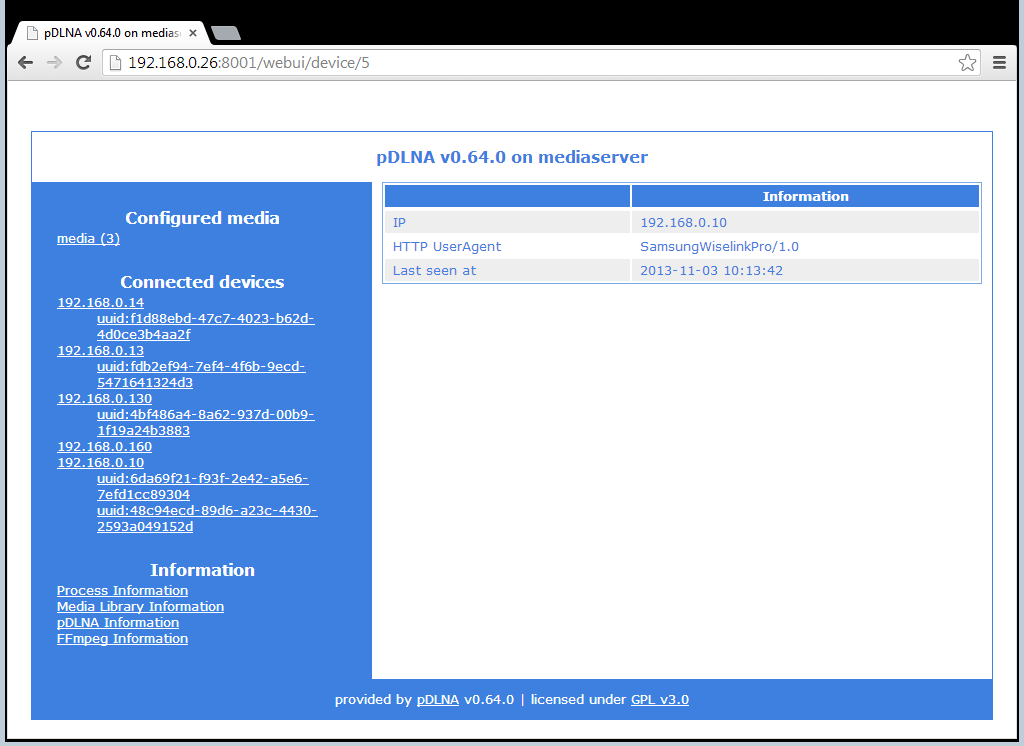
\includegraphics[width=34em]{images/webui_device_ip}
	\label{fig:webgui-connecteddevice-ip}
	\caption{WebUI: Information about a connected device per IP address}
\end{figure}

Figure~\ref{fig:webgui-connecteddevice-service} shows information, including the friendly name, the device type or the device description URL, after clicking on a service UDN.

\begin{figure}[!ht]
	\centering
		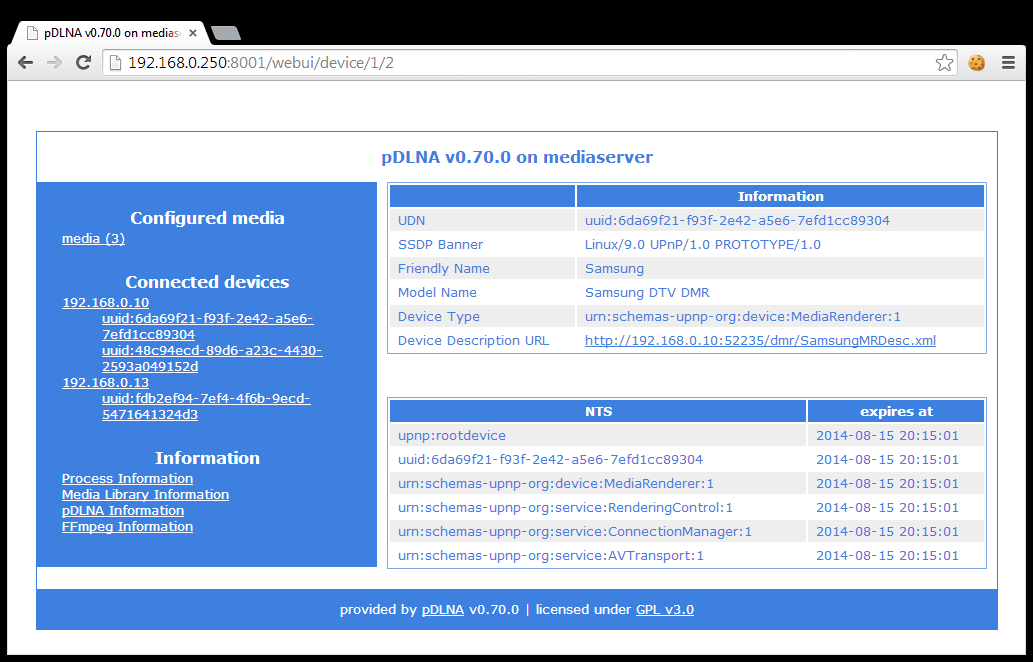
\includegraphics[width=34em]{images/webui_device_ip_service}
	\label{fig:webgui-connecteddevice-service}
	\caption{WebUI: Information about a connected device per service}
\end{figure}

\section{Information}

The third section in the navigation includes some various information about the running {\em pDLNA} installation.

While figure~\ref{fig:webgui-process} shows information about the process itself (including for instance memory and cpu usage), figure~\ref{fig:webgui-library} delivers information about the amount and size of media items included in the media library.

\begin{figure}[!ht]
	\centering
		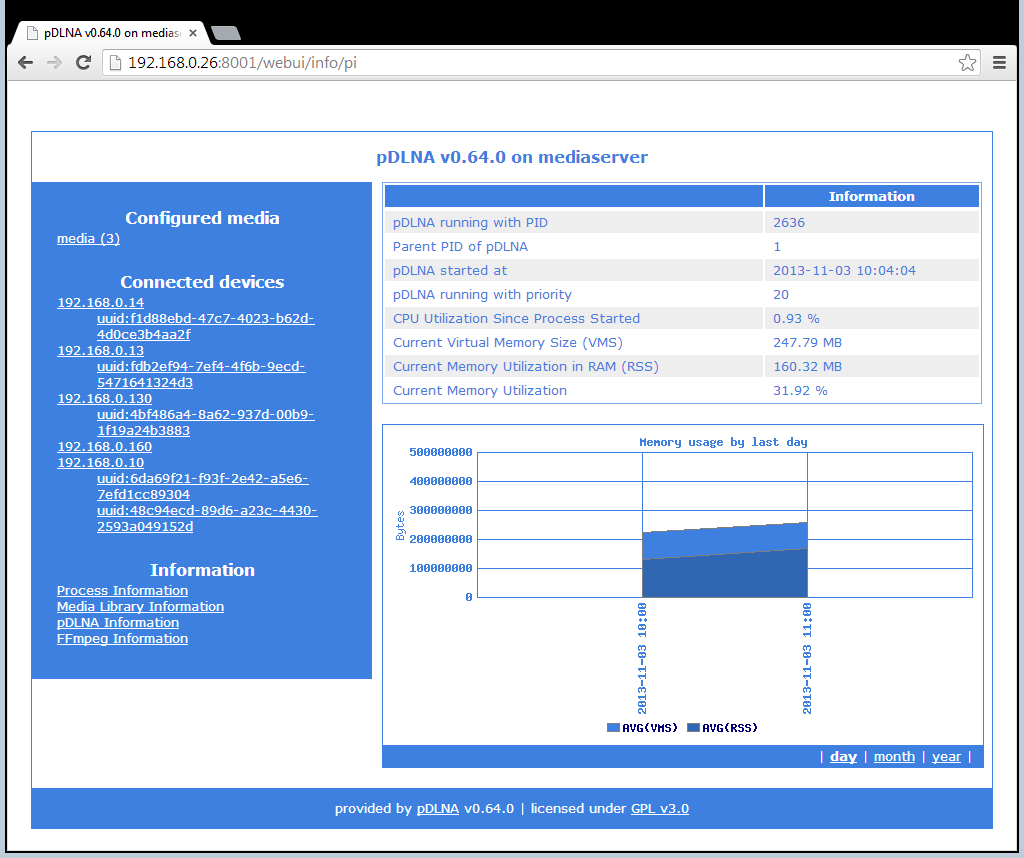
\includegraphics[width=34em]{images/webui_info_process}
	\label{fig:webgui-process}
	\caption{WebUI: Process Information}
\end{figure}

\begin{figure}[!ht]
	\centering
		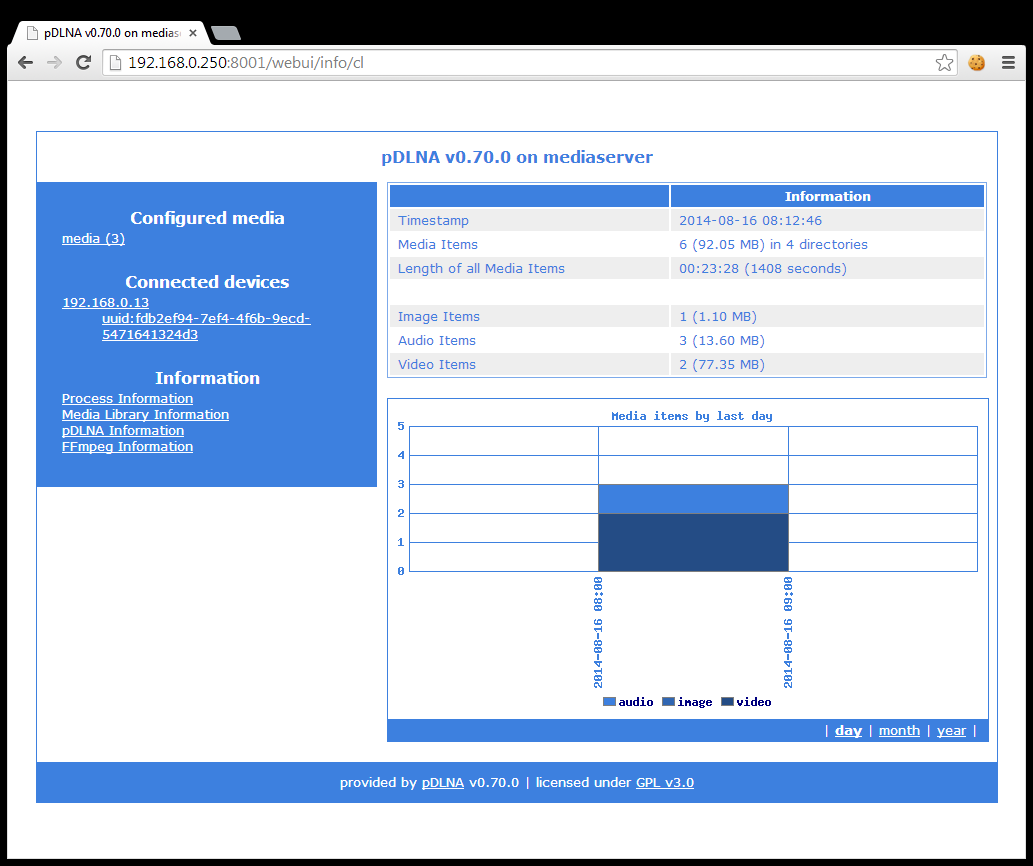
\includegraphics[width=34em]{images/webui_info_library}
	\label{fig:webgui-library}
	\caption{WebUI: Media Library Information}
\end{figure}

Additionally, the following figure~\ref{fig:webgui-pdlna} shows information about the installed {\em pDLNA} version and its release date. You are also able to execute a {\em Check4Updates}, which works as described in section~\ref{config-check4updates}, but shows the result in the WebUI.

\begin{figure}[!ht]
	\centering
		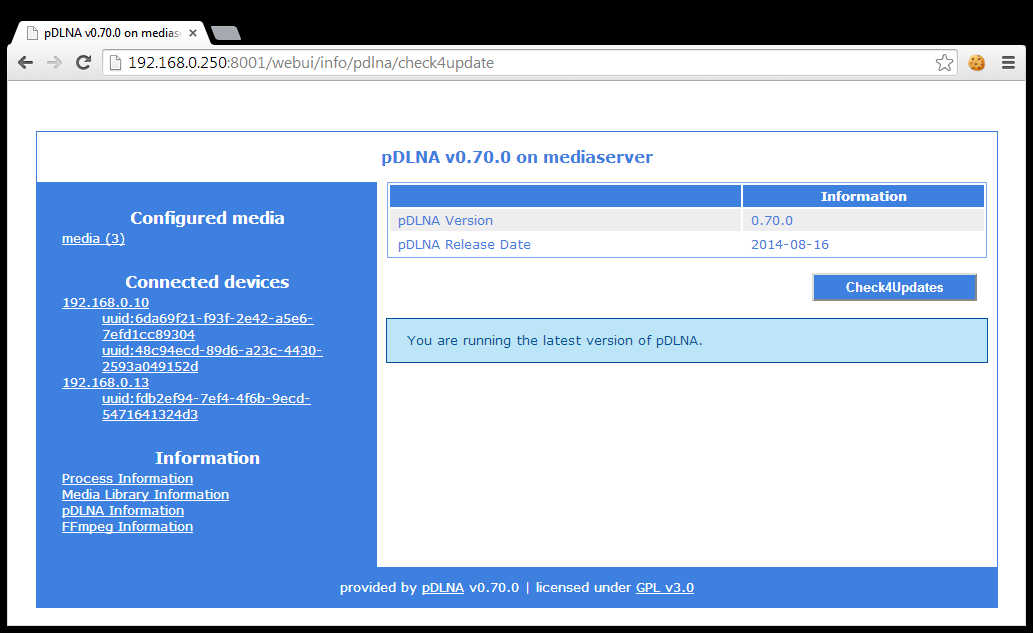
\includegraphics[width=34em]{images/webui_info_pdlna}
	\label{fig:webgui-pdlna}
	\caption{WebUI: pDLNA Information}
\end{figure}

And finally, the following figure~\ref{fig:webgui-ffmpeg} shows information regarding the used \verb|FFmpeg| installation, if the usage of \verb|FFmpeg| is configured.
% Temporary description
%This information provides easier access to supported transcoding profiles (see section~\ref{Transcoding_Profiles}).

\begin{figure}[!ht]
	\centering
		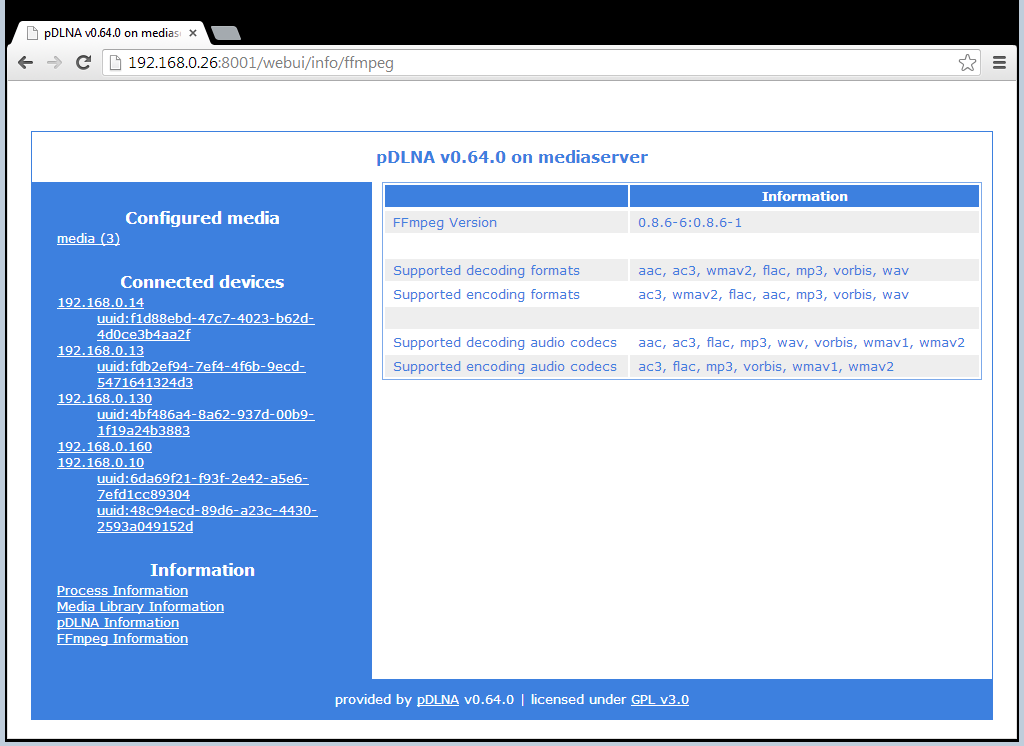
\includegraphics[width=34em]{images/webui_info_ffmpeg}
	\label{fig:webgui-ffmpeg}
	\caption{WebUI: FFmpeg Information}
\end{figure}